\documentclass[11pt]{article}
\usepackage[margin=1.1in]{geometry}
\usepackage{amsmath,amssymb,amsthm}
\usepackage{booktabs}
\usepackage{array}
\usepackage{tabularx}
\usepackage[protrusion=true,expansion=false]{microtype}
\usepackage[table]{xcolor}
\usepackage{enumitem}
\usepackage{titlesec}
\usepackage{tikz}
\usepackage{float}
\usetikzlibrary{arrows.meta,positioning,fit,calc,decorations.pathreplacing}
\usepackage{listings}
\usepackage{hyperref}
\hypersetup{colorlinks=true, linkcolor=blue!60!black, urlcolor=blue!60!black, citecolor=blue!60!black}
\usepackage[skip=0.6\baselineskip, indent=0pt]{parskip}

\titleformat{\section}{\large\bfseries}{\thesection.}{0.7em}{}
\titleformat{\subsection}{\normalsize\bfseries}{\thesubsection.}{0.6em}{}

\newcommand{\vmax}{V_{\max}}
\newcommand{\Tc}{T_{\mathrm{close}}}
\newcommand{\tx}[1]{\texttt{#1}}
\newcolumntype{L}{>{\raggedright\arraybackslash}X}

\lstdefinestyle{script}{
  basicstyle=\ttfamily\small,
  columns=fullflexible,
  keepspaces=true,
  breaklines=true,
  frame=single,
  framerule=0.3pt,
  xleftmargin=1em,
  escapeinside={(*}{*)},
}

\newtheorem{assumption}{Assumption}

% tables: a little more room between rows, and every other row shaded, so
% that rows of wrapped text stay distinct
\renewcommand{\arraystretch}{1.3}
\rowcolors{1}{}{black!5}

\definecolor{coop}{RGB}{232,245,233}
\definecolor{chainc}{RGB}{255,228,225}
\definecolor{proofc}{RGB}{230,240,255}

\title{\textbf{Lichen}\\L2s In CHannels ENforced by bitcoin}
\author{waxwing}
\date{Draft, October 2026}

\begin{document}
\maketitle

\begin{abstract}
A \emph{contract} with a hub lets a user hold the hub's tokens on a layer 2 and
withdraw them as bitcoin without trusting the hub for honesty or liveness. The L2 tokens are collateralised by the bitcoin in the user-hub multisig output\footnote{This can be embedded into a full Lightning channel, or a single isolated contract; both work.}, and if the hub refuses a withdrawal, or cannot answer because it is offline, it is enforced on Bitcoin. The only assumptions are those of the layer 2 itself, kept apart from the hub. No change to Bitcoin's
consensus is required. A withdrawal is a claim that a program, the withdrawal statement, ran on some input and produced an output: the statement is proved with RISC Zero and wrapped in Groth16, and a disputed claim is settled on Bitcoin by BitVMX~\cite{bitvmx}, whose interactive search over the execution of a RISC-V program, here a Groth16 verifier, is the technical core of the design.  Withdrawals are executed cooperatively in the channel --- with overwhelming likeliness because the statement is deterministically verifiable in milliseconds --- or, otherwise, a refused one is played as BitVMX's on-chain search, pre-signed once per contract. The trustlessness gain is paid for with liquidity (with receiving ability only contingent on offered ``inbound'' from the hub, as in Lightning). The hub (but not user) must also stay live during normal operation, since an offline hub loses disputes by timeout. The design is built and measured on regtest: a real proof of the withdrawal statement is accepted by BitVMX's unpatched Groth16 verifier in 478 million steps, implying about 22--25 transactions of 8-ary search on chain in the dispute's worst case.
\end{abstract}

\tableofcontents

\section{Introduction}

\subsection{Obvious objections to Lichen and why they're mostly wrong}

\paragraph{One central hub is dangerous.} If the hub disappears, the user gets the money. The hub cannot Sybil attack users by printing tokens fictitiously; the honest users' money is all backed. The only remaining risks are inherent to the L2 itself (is it a validity rollup or a quorum? Does it inherit finality from Bitcoin or is finality weaker? Etc.)

\paragraph{Bridges usually mean you can only withdraw a fixed size utxo, meaning operators and relying on swaps. Surely that applies here?} No. The withdrawal amount is encoded in bits in the bitcoin transaction witness, in dispute. This allows us to withdraw arbitrary amounts via multiple outputs of certain denominations~[\ref{sec:outcomes}].

\paragraph{Don't these constructions usually require a 1 of n honesty assumption from a signing committee?} Not here: we avoid this by the LN-GAP~\cite{lngap} trick: the contract is a \emph{bilateral} contract between the hub and each user; the presigning happens between them, just as in Lightning.

\paragraph{But if a bunch of users open channels with a hub, they can just .. pay each other through the channels?} A correct critique, partly, \underline{if} the L2 ledger doesn't do anything but plain payments. Even then, you would avoid receiver liveness being needed, avoid routing and other minor things. But the real answer is: the L2 can offer more functionality. It can use zcash style shielded notes, allowing very high privacy while staying in the L2. It can also (in a different ``lichen'' on a different hub) offer rich smart contracting, etc.

\paragraph{But this an IOU/ hub's token, so it's not actually bitcoin.} Incorrect with a crucial caveat. See the first point: every sat is redeemable via the user-hub contracts, \emph{without} the hub's permission, one-to-one, so these are actually bitcoin \emph{but only as long as you have liquidity to receive them}. A new user on L2 without a contract with the hub, or a user holding a balance on L2 far in excess of their inbound liquidity in their own contract, is holding \emph{credit}, and has no such guarantee. But that's their choice.

\paragraph{But still, a single central hub feels like bad design. Why not multiple hubs?} It's because of what these L2 tokens are. They are fungible, \underline{enforceable} claims on the hub's money; they are minted by the hub itself, just on its own say-so. If you had hub 1 and hub 2, those claims are not transferrable trustlessly to the hubs themselves. If hub 2 prints a billion sats out of nothing and users accept it on the L2 they can redeem it with hub1, leaving hub1 out of pocket. From this line of thinking we see an interesting comparison with ecash servers: the hub can print as much as it likes, but it cannot steal/``rug''.

\paragraph{So what's the catch?} The negatives are twofold: one is liquidity, and this is easy to understand as the analog of the inbound liquidity pain point in Lightning, because it's basically the same thing. Such a hub \emph{can} give no inbound liquidity to a user: they get tokens on L2 to spend, but they cannot (safely) receive. If they receive, it's just credit that someone else will hopefully buy from them. But the design does not assume that, of course, it allows receiving up to a ``cap'': the user negotiates that extra potential receiving amount (inbound liquidity) when it sets up the contract with the hub. The second negative is very concrete, and is a design decision rather than an absolute requirement: we use BitVMX's bisection (in fact 8-ary not binary) to enforce that the ZKP is valid, on-chain. In the worst case this is 20-25 transactions and may require watchtower design to be easy enough for users to fully rely on. In a correctly built implementation this is exceptionally rare because the incorrect party (trivially established) is guaranteed to pay all the fees (up to its reserve), and lose money.

\subsection{A note on the delta to LN-GAP}
\label{sec:family}

LN-GAP\cite{lngap} puts contracts governed by arbitrary programs into Lightning~\cite{lightning}
channels: a contract's outcome is decided by a game whose moves are
signed off-chain, with pre-signed transactions that let either party
take a dispute to Bitcoin~\cite{lngap}. Lichen mainly differs in trying to achieve trustlessness at the expense of LN-GAP's O(1) onchain resolution; a tradeoff that fits well with the intent of creating \emph{an L2 from a bunch of channels with a hub}:

\begin{center}
\small
\begin{tabularx}{\linewidth}{p{24mm}LL}
\toprule
& LN-GAP &  Lichen  \\
\midrule
venue & trusted: a majority of members attests moves & none \\
a dispute is decided by & the venue's attestations  & the chain: BitVMX's search \\
suited to & interactive games where time has value  & withdrawals from a hub's layer 2 \\
on-chain cost of a dispute & constant & steps on chain log(program length) \\
\bottomrule
\end{tabularx}
\end{center}

\paragraph{Why Lichen needs no venue.}  What if the ``game'' the two sides are playing is a fixed, deterministic adjudication of truth? Timing doesn't really matter as much, just ensured completion. Secondly, the actual game playing is going to be a rare back-out clause: unlike say, chess, in which the winner is not predictable at the start, so that the game is the point. If the ``game'', as here, only exists to prevent cheating and can only play out in one way, it's more important to achieve trustlessness, even at cost of a lot more onchain execution, because that cost won't usually need to be paid and the value of real trustlessness is immense.

\section{Contracts with the hub}
\label{sec:terms}

\textbf{Alice}, the user, has a contract with a \textbf{Hub}, instantiated as a 2 of 2 output in a channel between them, or
on its own (Section~\ref{sec:contract}), with these terms:
\begin{center}
\small
\begin{tabularx}{\linewidth}{p{16mm}L}
\toprule
$D$ & Alice's deposit: she puts $D$ bitcoin in and receives $D$ of the hub's tokens on the L2 \\
$\vmax$ & the most she can withdraw: her $D$ and the hub's liquidity $\vmax - D$ \\
$r_A, r_H$ & the \emph{contract reserves}, Alice's and the hub's: returned in every honest outcome, forfeited to the other side by losing a dispute (Section~\ref{sec:outcomes}); the contract holds $\vmax + r_A + r_H$ \\
$b$ & the amount she withdraws, by returning $b$ tokens to the hub on the L2 with the memo $c$ \\
$c$ & the contract's identifier, its memo \\
$\Tc$ & the contract's end: with no withdrawal by then, the hub takes it \\
\bottomrule
\end{tabularx}
\end{center}
Every token is a liability of the hub, collateralised by the contract of whoever holds it, within that holder's cap; within $\vmax$ and before $\Tc$, Alice trusts the hub for nothing, not even to be online: a withdrawal it does not answer is paid by timeout. The hub's provided liquidity is the sum of its users'
$\vmax - D + r_H$.

\begin{figure}[H]
\centering
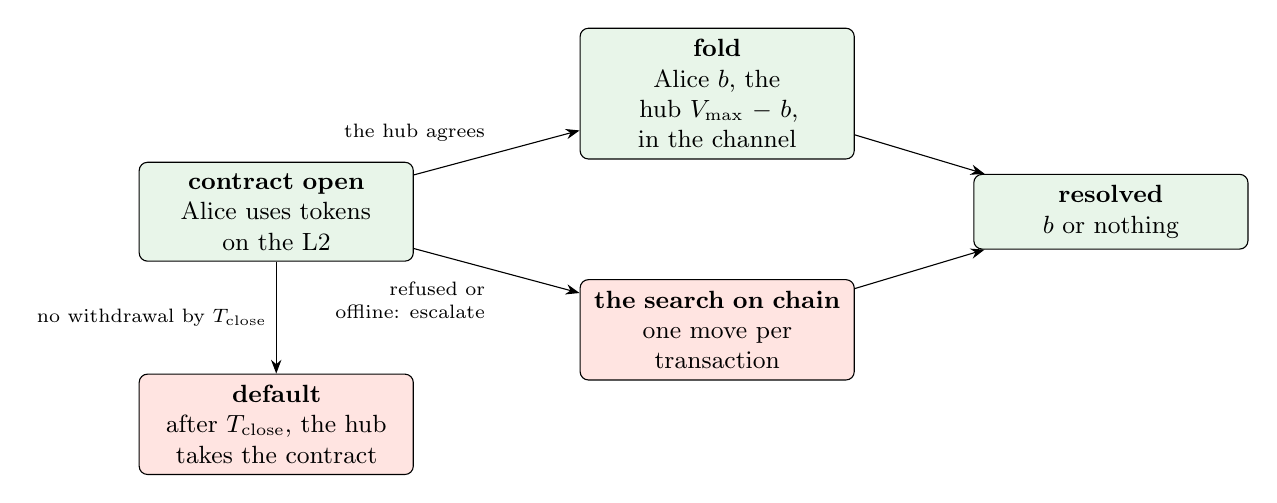
\begin{tikzpicture}[
  font=\small,
  st/.style={draw, rounded corners=3pt, align=center, inner sep=4pt, text width=#1},
  st/.default=32mm,
  >={Stealth[length=5pt]},
]
\node[st, fill=coop] (live) at (0,0) {\textbf{contract open}\\Alice uses tokens\\on the L2};
\node[st, fill=coop] (fold) at (5.6,1.5) {\textbf{fold}\\Alice $b$, the hub $\vmax - b$,\\in the channel};
\node[st, fill=chainc] (ladder) at (5.6,-1.5) {\textbf{the search on chain}\\one move per\\transaction};
\node[st, fill=chainc] (def) at (0,-2.7) {\textbf{default}\\after $\Tc$, the hub\\takes the contract};
\node[st, fill=coop] (end) at (10.6,0) {\textbf{resolved}\\$b$ or nothing};
\draw[->] (live) -- node[above left=1pt, font=\scriptsize] {the hub agrees} (fold);
\draw[->] (live) -- node[below left=1pt, font=\scriptsize, align=right] {refused or\\offline: escalate} (ladder);
\draw[->] (live) -- node[left, font=\scriptsize] {no withdrawal by $\Tc$} (def);
\draw[->] (fold) -- (end);
\draw[->] (ladder) -- (end);
\end{tikzpicture}
\caption{The life of a contract. Green states stay off-chain or settle
cooperatively; red states are on chain.}
\label{fig:life}
\end{figure}

\section{How a withdrawal from the L2 is proved valid}
\label{sec:statement}

\subsection{The statement proved}

For brevity we have not yet given a description of what the L2 looks like, but its main features are here, to explain the proof structure.

The L2 is a ledger of notes, with state updates signed by a sequencer\footnote{We'll talk more about achieving finality via Bitcoin or otherwise later~[\ref{sec:finality}].}. A note is an owner, a value, a memo and a
random $\rho$, which makes every note distinct (two equal payments to the
same owner are still two notes); its commitment is a SHA-256 hash of
these, and the commitments form an append-only Merkle tree. A spent note
is not removed from the tree, which would change every other note's
path, but recorded by its \emph{nullifier}, a hash of its commitment, in
a set the sequencer keeps: spending a note twice repeats its nullifier.
So a note's path under a root stays valid however the ledger moves on.
This description may confuse a little, but we're trying to avoid adding the complexities of shielding a la Zcash designs \emph{now}, for the proof of concept phase; but we intend to add something in that style: in that case, $\rho$
also hides the note's contents, and the nullifier is derived from a
secret key so that nobody can link it to its note. A
state root $R$ hashes the height, the tree's root and the nullifier
set's root, and the L2's sequencer signs it (BIP340). The statement therefore is:
\begin{quote}
``a note owned by the hub, of value $b$ and memo $c$, is in the
commitment tree of a state root the sequencer signed''
\end{quote}
Its public output, the \emph{journal}, is $b \,\|\, c$. The program created to generate these proofs has what's called an ``image id'', which includes both sequencer and hub keys (remember, only the hub can mint L2 tokens).

\subsection{From a program to a verifiable claim}

\begin{figure}[H]
\centering
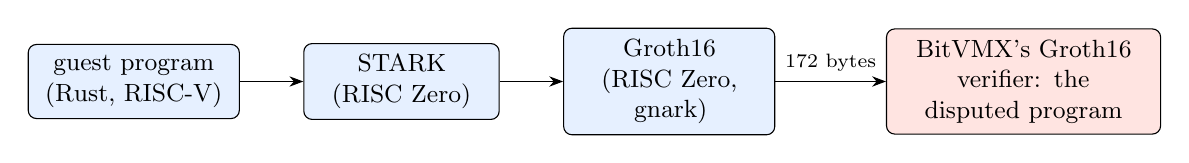
\begin{tikzpicture}[
  font=\small,
  box/.style={draw, rounded corners=3pt, align=center, inner sep=4pt, text width=#1},
  box/.default=27mm,
  >={Stealth[length=5pt]},
]
\node[box=24mm, fill=proofc] (g) at (0,0) {guest program\\(Rust, RISC-V)};
\node[box=22mm, fill=proofc] (s) at (3.4,0) {STARK\\(RISC Zero)};
\node[box=24mm, fill=proofc] (w) at (6.8,0) {Groth16\\(RISC Zero, gnark)};
\node[box=32mm, fill=chainc] (v) at (11.3,0) {BitVMX's Groth16\\verifier: the\\disputed program};
\draw[->] (g) -- (s);
\draw[->] (s) -- (w);
\draw[->] (w) -- node[above, font=\scriptsize] {172 bytes} (v);
\end{tikzpicture}
\caption{The withdrawal statement runs in RISC Zero's zkVM; its proof is
compressed to a Groth16 proof; a dispute is over the execution of a fixed
RISC-V program that verifies it~\cite{risc0,bitvmx}. A companion note
explains each stage~\cite{pipeline}.}
\end{figure}

So the disputed program is always the same: the Groth16 verifier that
FairgateLabs compiled for BitVMX~\cite{bitvmxcpu}, unpatched. Its input is 172 bytes, read as 43
four-byte words, each signed by Alice with its own one-time key when she
makes her claim:
\begin{center}
\small
\begin{tabular}{lll}
\toprule
words & content & used by the contract \\
\midrule
0 & the journal's length (2) & checked \\
1--8 & the image id & checked against the pinned statement \\
9--40 & the proof's three points\footnotemark , compressed & by the search only \\
41 & $b$ & read by the payout \\
42 & $c$ & checked against the contract \\
\bottomrule
\end{tabular}
\end{center}
\footnotetext{A Groth16 ZKP always consists of exactly 3 elliptic curve points, around 100-200 bytes depending on compression serialization.}

The checks are the hub's leaves on the contract: Alice's signature on a
word with the wrong value gives the hub the contract. The image-id check
is essential: without it, Alice could submit a valid proof of a
\emph{different} program, which the verifier would accept.

\section{Building blocks}
\label{sec:blocks}

More detail on the contract \emph{construction}. We're thinking of a single output (utxo), 2-of-2 controlled by Alice and the Hub, which is taproot and so can have several spending conditions encoded in leaves of the taproot tree. Apart from the normal segwit trick of pre-signing transaction chains, leaving the witness chooseable after the fact, there are two main building blocks:

\subsection{Values that Script can read: one-time signatures}

Bitcoin Script can check a signature only on the spending transaction,
never on a message of the signer's choosing. A contract that must act on
a value a party chooses later (Alice's $b$, a move in the search) uses
Winternitz one-time signatures, which Script verifies by hashing alone,
leaving the signed digits on the stack to compare~\cite{bitvm,bitvmx}. The
keys are exchanged when the contract opens, one per value, each used
once; signing two different values under one key is
\emph{equivocation}, which a leaf can prove, giving the signer's stake
to its counterparty.

\subsection{BitVMX's search}
\label{sec:search}

BitVMX~\cite{bitvmx} is the main workhorse tech in this design. BitVMX-CPU settles a claim about a RISC-V program's run. The rest of the design details arrange the conditions
under which BitVMX's search can serve as the backstop of a withdrawal,
using its emulator, search and verifier, with two bug fixes and the authenticated jump list added in a fork~\cite{bitvmxcpu,bitvmxfork}. The prover (here Alice) claims that the program, on her input, halts
after $n$ steps with a given exit code; each step's write is hashed into
a chain, and she commits to the last hash. If the verifier (the hub)
disagrees, they search: in each round the prover posts the hashes after
$k - 1$ evenly spaced steps of the interval in dispute, and the verifier
names the segment it disputes. With $k = 8$, ten rounds cover the
verifier's $2^{29}$ steps. They end agreeing on the hash after one step,
$t$, and disagreeing on the hash after the next. The prover then posts
her record of step $t + 1$: the instruction, the values it reads (and
the step that last wrote each) and writes, and the hashes on either
side.

Every move is its mover's one-time signatures on the values it posts,
one key per field (the claim, each hash, the choice, the record, each
step hash), and nothing else. Nothing about the search's state is
signed: a rule re-reveals the signatures it reads, which are public once
posted, and derives what it needs, as BitVMX's own scripts do. Alice's
\emph{proof} of the disputed step, one pre-signed leaf for each class of
instruction, runs BitVMX's verification script for the instruction on
her record and checks the step hash. The hub's \emph{disproves} are
BitVMX's challenges: the agreed step must be the hub's choices
concatenated, the step hashes must be those Alice posted for steps $t$
and $t + 1$ in the search (an \emph{equivocation} challenge for each
round and index), the record must agree with the program (the opcode at
its pc, the entry point, the pc the previous step wrote, the memory
sections) and its never-written reads with the input or the initial
data, and a claimed success must end in a success exit
(\tx{halt\_exit}).

\paragraph{Reads.} The step hash covers what a step writes, not what it
reads: a read's value is whatever was last written to its address. So
Alice could claim a false value for a read, naming a plausible step as
its last write, and execute the instruction faithfully on it: her chain
would diverge at that step, the search would find it, and her proof
would pass. BitVMX catches this with a second search for the read's last
write, as long again as the first. Here the trace is hashed instead as
an \emph{authenticated jump list} (S.~D.~Lerner~\cite{bitvmxinnov}):
\[
  h(i) = \mathrm{BLAKE3}\big(h(i-1) \,\|\, h(\mathit{jump}(i)) \,\|\,
  \mathit{write}_i \,\|\, i\big),
\]
where $\mathit{jump}(i)$ is an earlier step chosen by the step number
alone, so that any step reaches any earlier one in a few times
$\log_2 n$ hops, each to the previous step or to the long jump (at most
86 for $2^{29}$ steps, about 52 on average). A genuine hash commits to its
step number, so its back-links are the genuine hashes of the steps it
names. To show a false read, the hub posts the hashes along a path from
the agreed $h(t)$ back to the last write, and the write's preimage; its
verdict wins if the write there contradicts Alice's read (another value
at the step she names, or a later write to her address). Alice, holding
the true history up to $t$, may challenge any hop whose hash she finds
false; the hub must then reveal that step's preimage, which must hash to
the posted hash and link back to the next, so a forged path loses at its
first false hop. The same machinery settles one more lie a jump list
makes possible: Alice's disputed step commits to the hash of its long
jump, and a false one would let a valid write prove on a false chain; the
hub's path to $\mathit{jump}(t + 1)$ shows the true hash. This is one
round where BitVMX needs a second search: about three more transactions
(Section~\ref{sec:ladder}).

\section{The contract logic}
\label{sec:contract}

\subsection{Three ways out}

A contract ends in one of three ways; its output, in each
commitment, carries two leaves for them besides Lightning's revocation:
\begin{itemize}[leftmargin=1.5em]
\item the \emph{fold}: a cooperative update of the channel (Alice
  $b + r_A$, the hub $\vmax - b + r_H$), the normal case, nothing on
  chain;
\item \tx{default}: after $\Tc$, a transaction pre-signed at the
  contract's opening pays the hub $\vmax + r_H$ and returns Alice's
  reserve $r_A$. This is the liveness requirement on Alice: turn up at the end, i.e. it's a very low bar requirement; whereas the hub must always be ready to answer disputes.
\item \tx{escalate}: Alice's claim goes on chain as the first move of
  BitVMX's search, with her signed input words, and the search
  continues on the \emph{dispute chain}. This will almost never happen, because given Alice's proof, the hub can calculate $\sim$ immediately that he's guaranteed to lose, so just pays out cooperatively (\emph{fold} as above).
\end{itemize}

\paragraph{In a channel, or on its own?} A contract can be a standalone
output, a 2-of-2 between Alice and the hub with the same two leaves,
opened by one on-chain transaction and folded by another (a cooperative
key-path spend paying $b + r_A$ and $\vmax - b + r_H$). Putting this output in a Lightning channel is an efficiency layer: in it the fold is a channel update, collateral can be reallocated and contracts renewed without touching the chain, and
deposits can arrive as Lightning payments; the price is that every channel update re-signs the contract's pre-signed transactions, for both commitments. The proof of concept uses the standalone form; earlier LN-GAP code demonstrates contracts embedded in channel commitments, with revocation; it could be applied here.

\subsection{The dispute chain}
\label{sec:ladder}

Remember that in dispute we do a search over the execution trace of a program, which is actually a Groth16 verifier.

The dispute search alternates Alice's rounds of hashes and the hub's choices:
with an 8-ary search over the verifier's $2^{29}$ steps, ten rounds and
21 moves. On the dispute chain each move is a transaction spending the previous
one. Each of the chain's outputs has two pre-signed spends: the
\emph{post}, by which the next mover publishes its signed move and
creates the next output, and the \emph{timeout}, valid $w$ blocks later,
which settles the dispute against the party that failed to move. Each
output also carries the other side's rules on the move just made (a
choice out of range, Alice's; the final record's challenges, the hub's),
and the last step is proved in Script.

\paragraph{A move.} A move is its mover's one-time signatures on what it
posts, one key per field: Alice's round of seven hashes, about 7.5~kvB;
the hub's choice, a byte, about 0.3~kvB; her final record and its hashes,
about 6.8~kvB. A key per field keeps the rules within Script's stack:
the stack holds at most 1,000 items, the witness counted, and a signed
byte costs four (two digits and two chain values), so a rule can
re-reveal only a few hundred signed bytes, and re-reveals only the fields
it reads.

\paragraph{What the other side must learn from the chain.} Each party
runs its own emulator and sees nothing of the other's but what is on
chain, so everything it needs to play and to disprove must be published
there, under the other's signature. Three things are: move~1 signs the
claim (the claimed last step and final hash) with round 1's hashes, and
the final move signs the disputed step's record; and the hub, to execute
the program at all, needs Alice's whole input, of which the escalation
carries only the words the payout and the checks read. When those don't
cover the input, an \tx{inputs} link follows the escalation with the
rest of her signed words (32 for the Groth16 verifier), before the hub
must move; if it does not come within the window, the hub's timeout
takes the contract.

\paragraph{Pre-signed once.} Each step is a 2-of-2 transaction
pre-signed when the contract is opened; the move travels in the witness,
which a transaction's id does not cover, so every step's id is fixed in
advance and the next can be signed against it. Pre-signing binds a
transaction to the exact outputs it spends, so a pre-signed chain can be
shared only by paths that reach it through the same transaction. Here
there is one: \tx{escalate}. So the dispute chain is pre-signed once, linear in
the search's length: about two transactions a move, the final step's
proofs (one per instruction class, pre-signed so that a proved
withdrawal pays $b$), and the read and jump challenges' set
below.

\paragraph{Optional off-chain play.} The parties may still play the
search off-chain by agreement, exchanging signed moves; if either stops,
the other escalates and \emph{replays} the moves already made from the
signatures it holds, then play continues on chain. Since each move is
signed alone, the escalator could replay one of its own moves other than
the one its opponent answered. But it would have signed two values under
one key: every dispute chain output carries an \tx{equiv\_d} leaf for each key
of each move so far, by which the other side shows the two signatures
and takes the output at once, ahead of any disprove, which waits
$\delta$. So replay is faithful.

\paragraph{Fees.} A link of the dispute chain (the escalation, a move)
must keep its transaction id, since the next link was signed against it,
so nothing can be added to it. It is an ordinary transaction paying a
floor of 1~sat/vB of its own out of the contract, so that it relays
alone, with an \emph{anchor}, an output only its poster can spend; the
poster tops the fee up with a child spending the anchor and a coin of
its own. The opponent's next move waits a block after the link confirms
(\tx{post} carries \texttt{1 OP\_CSV}), so nothing but the poster's child
can sit on an unconfirmed link: the challenge and response happen on the
chain, not in the mempool, and the pinning that TRUC's mempool rules
exist to prevent has no handle here. A link may then be as large as
relay policy allows (100~kvB), where TRUC caps it at 10~kvB: the 8-ary
escalation is 9--12~kvB, a path's chunks up to 93~kvB. The floors come
out of the loser's reserve. Each is sized as if the leaf its link spends
sat at its tree's greatest depth (which leaves are deepest depends on
their hashes, and so on the keys), so the floors are a property of the
statement, fixed before any contract opens: on the Groth16 verifier the
deepest dispute, a worst-case read, has 195,411~sats of them at
1~sat/vB, half of it the path's combine. A transaction that ends the chain (a
timeout, a proof, the default) is spent only by runtime leaves, so its
id may change: both signatures on it are \texttt{ALL|ANYONECANPAY},
committing to its own input and all its outputs, and the broadcaster
adds a coin as an input. The feerate is chosen at broadcast rather than
guessed at signing, beyond the links' floors. The prices are the usual
ones: a party keeps fee coins (a coin added to a transaction whose
outputs are fixed has no change), and the floors are paid whatever the
feerate.

\paragraph{The read and jump challenges.} A path (Section~\ref{sec:search})
of up to 86 hashes, 1,720 signed bytes, does not fit one input's stack,
which holds about 250. So it is posted in chunks, one per input of a
single transaction: from the final record's output, the hub's
\tx{path\_split} makes eight \emph{carriers} (the first holding the
value, the rest dust), and \tx{combine\_$k$} spends the first $k$ of
them, chunk $c$ in input $c$ (the first chunk holds the hops' count,
their types, the path's end and 8 hashes; each other 11). Both are
pre-signed, a combine for each $k$. After the combine, Alice may post her
choice of a hop to challenge; after her window, the hub's verdict
(\tx{jump}, \tx{read\_$r$}) takes the output with the end's preimage;
after her choice, the hub's reveal of that hop does, or Alice's timeout
pays her. If the hub splits and never combines, the first carrier's
timeout pays her; the hub sweeps the other carriers, dust, at leisure. A
read dispute adds three or four transactions to the search.

\subsection{Outcomes}
\label{sec:outcomes}

The search only ever decides Alice's withdrawal: $b$ if her claim
stands, nothing if it fails; the rest of $\vmax$ goes to the hub. The
reserves follow the dispute: the loser's goes to the winner, whether it
lost by a disprove, a failed input-word check, \tx{equiv\_b}, or by not
answering in time. A disprove, a runtime spend, pays the disprover the
whole output: it fires only on a provable lie, so the liar loses.

\paragraph{Paying $b$: the bit outputs.} When Alice wins, the payout
must send her $b$ (as built, rounded down to 512~sats: bits below $2^9$
have no output), a value she chose when she claimed; but the
payout is pre-signed, so its amounts are fixed, and Script cannot
compute an amount. One pre-signed transaction per possible $b$ would be
too many. Instead, as for numeric DLCs~\cite{dlcnumeric}, the payout
decomposes $b$ in binary: for a unit $u$ and $K$ bits ($2^K u > \vmax$),
output $i$ holds $u\,2^i$ and has three leaves:
\begin{center}
\small
\begin{tabular}{lll}
\toprule
leaf & spent by & condition \\
\midrule
Alice's & Alice, after a delay $\delta$ & her one-time signature on $b$ (word 41) has bit $i$ set \\
the hub's & the hub & the same signature has bit $i$ clear \\
\tx{equiv\_b} & the hub & two signatures on different values of $b$ \\
\bottomrule
\end{tabular}
\end{center}
Since $b$ is under a one-time key, the bits Alice can claim are those of
the single value she signed, and their outputs sum to $b$; the hub takes
the rest. For $b = 9$ she takes outputs 0 and 3. Her leaf waits $\delta$
so that the hub can show an equivocation first. With $\vmax = 0.1$~BTC
and $u = 1000$~sat, $K = 14$; each output's spend is about 300~vB, and
each party can sweep its outputs in one transaction. The reserves sit in
one more output, paid to the winner, with an \tx{equiv\_b} leaf of its
own. In the cooperative fold none of this appears: the channel simply
pays $b$.

\paragraph{The contract reserve.} A reader who knows Lightning will see
a familiar question here. Lightning's penalty deters publishing a
revoked state only if the cheat has something to lose: a party whose
balance has been drained to nothing can publish an old state for free
and profit if its counterparty is not watching, which is why channels
keep a \emph{channel reserve}. A contract without reserves has the same
hole, on both sides, though not where one might first look:
\begin{itemize}[leftmargin=1.5em]
\item What Alice risks by a false claim is not her deposit $D$ but her
  honest outcome, the return $b$ she could actually prove. Once she has
  spent her tokens on the layer 2 that is nothing, and a claim of
  $\vmax$ becomes a free option on the hub being offline. It is cheap to
  hold: she escalates, and if the hub answers she simply stops and loses
  by timeout what she would not have had anyway.
\item The hub makes no claims; it refuses and challenges. Losing the
  search costs it only fees, since its honest outcome is what it is left
  with anyway. So it can refuse a valid withdrawal and hope that Alice
  cannot play the search in time, whatever it committed to the
  contract.
\end{itemize}
So the quantity that matters is not what each party put in but what
each loses by losing a dispute, and the remedy is a reserve on each
side that only a lost dispute moves. Sizing follows the same logic as
Lightning's. A probe that succeeds with chance $p$ (the hub is offline)
gains up to $\vmax - b$ and otherwise costs the reserve, so it is
unprofitable when
\[
  (1-p)\, r_A > p\,(\vmax - b), \quad\text{that is, for every } p < \frac{m}{1+m} \text{ with } r_A = m\,(\vmax - b).
\]
A reserve can therefore deter probing as firmly as one likes, at a price
in locked capital: $m = 1\%$, about a channel reserve, deters only a
probe with less than a 1\% chance; $m = 1$ one with less than even
odds; $m = 5$ anything short of near-certainty that the hub has lost
its keys. Nobody would lock several times their stake to hold a contract,
just as nobody would keep a channel reserve of 500\%; the practical
choice is where to sit on that curve, and it depends on what the
parties know of each other. A floor is clear in any case: every
abandoned probe and every refused valid withdrawal should cost the one
who started it at least the other side's dispute fees, so that griefing
is paid for by the griefer. Part of those fees is known when the
contract is signed: the links' floors, which reach 195,411~sats in the
deepest dispute on the Groth16 verifier (Section~\ref{sec:ladder}), so
neither reserve should be smaller. lichen's hub takes for its own the
larger of its share of the cap and that figure. The first defence stays what it is in Lightning: the hub is
live because that is its business, and Alice, the occasional absentee,
is the one a reserve protects. The price is capital (Alice brings
$D + r_A$, the hub $\vmax - D + r_H$) and severity: an honest party who
starts a dispute and then disappears loses its reserve as well.

\paragraph{Who it suits.} A reserve is locked, not spent: an honest
party gets it back in every outcome (the fold, the default, a dispute it
wins) and loses it only by losing a dispute, which for an honest Alice
means going absent in the middle of one. So nothing stops a small
balance with a large reserve; Alice pays only in liquidity. The binding
cost falls on the hub. Its reserve must make Alice whole when it refuses
her withdrawal and loses, so it must cover her worst-case dispute,
however small her balance: about 195~kvB on the Groth16 verifier, which
is 195,000~sats in floors at 1~sat/vB, 400,000 at 2~sat/vB, two million
at 10. On top of that the hub locks the cap's headroom $\vmax - D$. A
user holding 50,000~sats therefore costs the hub about as much locked
capital as one holding two million, and earns it less. Alice's own
reserve is the hub's to demand, and a hub can ask a small user for less
at the price of some exposure to probing. The design therefore suits
balances from about half a million sats, and comfortably from a few
million, where these reserves are a few percent of the stake. Large
balances raise no new cost in the contract: the dispute does not grow
with $b$, whose binary payout only adds outputs. What grows is the
trust placed in the layer 2's finality, which anchoring its roots on
Bitcoin addresses (Section~\ref{sec:finality}). A contract's amounts
are 32-bit counts of a unit, so with a unit of one satoshi a contract
holds up to about 42.9~BTC.

\section{Finality from Bitcoin}
\label{sec:finality}

With a single, or indeed a distributed, sequencer signing updates to L2 state, without a consensus mechanism like proof of work or proof of stake, it's free to ``rewrite history'' for transactions on the L2, enabling double spend attacks. The techniques used in ETH L2s to handle this involve the rollup data publication and contract state on the base chain; that is not available here. So in the absence of proposing expensive consensus on L2, it makes the most sense to inherit finality from Bitcoin, as Shielded CSV~\cite{shieldedcsv} and Shielded Bitcoin~\cite{shieldedbtc} do (the first by publishing each transaction's nullifier on Bitcoin, the second by publishing every transaction there in full), but here using the single use seal concept~\cite{toddseals}, with one commitment per batch.

If each sealed batch's root is committed in a Bitcoin transaction that spends the previous batch's commitment output, a fork of the layer 2 needs a double spend on Bitcoin. It costs one small transaction per batch, not per layer 2 transaction. A committee of sequencers then needs only one honest member for inclusion (members append batches in turn); forks are excluded by Bitcoin, not by a threshold.

What sealing does not provide is availability: a seal commits to a root, not to the data behind it. This paper \underline{does not} answer this question; it is a function of exactly how the L2 ledger is constructed (with a Bitcoin publication component, or not). But if data availability is not addressed, the user does have to trust the sequencer in a very concrete sense: if the sequencer refuses to provide the Merkle path for her return note, the user has no way to retrieve their funds in the contract, and loses them. This strongly argues for the above-mentioned ``committee of sequencers'', because you just need 1 to include your withdrawal and give you its path to be safe\footnote{A more advanced idea is publishing withdrawals on Bitcoin, requiring L2 to read L1 in a similar way to what is described next}.

In this scenario, Alice's withdrawal statement must then show that its root is sealed: a light-client/SPV proof inside the guest, a chain of block headers from a checkpoint to the block carrying the seal, with its Merkle path, and some confirmations after it. The checkpoint is a block hash pinned in the contract when it opens, checked as an input word like the memo; since
every withdrawal falls before $\Tc$, the chain a proof covers is bounded by the contract's lifetime, and a contract shorter than a difficulty period (2016 blocks) crosses at most one retarget, so the guest can bound each header's target by the checkpoint's within the protocol's factor of four.

\underline{The cost is surprisingly small}: a header is about three SHA-256 compressions, which RISC Zero accelerates, so a thousand headers are a few hundred thousand cycles, against the 5.9 million of today's statement.
The comparison is not like for like: today's statement uses no
acceleration (almost all its cycles are the sequencer's signature,
checked in plain software), while the headers' figure assumes RISC
Zero's SHA-256 circuit, 68 cycles a block~\cite{risc0accel}. Accelerated,
the statement itself should fall under a million cycles
(Section~\ref{sec:costs}), so a thousand headers would add perhaps a
quarter or a third to it; hashed in plain software, at a few thousand
cycles a compression, they would cost around ten million, more than
today's whole statement. The dispute is unchanged. In the cooperative case the hub checks seals with its own node.

Forgery then becomes a matter of mining a fork in Bitcoin itself. In current Bridge designs, like Union~\cite{union}, a challenger answers the claimant's chain with a
heavier one, which the claimant may dispute in turn, in a second BitVMX
game with the roles reversed.

But we don't want to or need to do that; the claimant is always the user and the dispute is settled on one statement.

So any forgery attack is on the side of the user; and such an attack to achieve maximum returns \emph{could} use it to steal from the hub across multiple contracts.
So the bound is not one contract's cap but
the hub's total headroom exposed to a single forged chain. As long as
that stays well below the reward of the blocks a fork must replace, the attack remains un-economic. This is the kind of security you can claim for Bitcoin itself, basically.

\section{Watchtowers}
\label{sec:watch}

A dispute runs for a day or more (about 140 blocks at $w = 12$, as built), and Alice must
answer each of the hub's moves within $w$ blocks. A laptop that sleeps
or travels will miss one, and a missed move loses the dispute and her
reserve. The natural answer is Lightning's: a \emph{watchtower}, a
service that plays her side of the search while she is away. Its moves
follow from her trace, which it can compute itself from her public
input. The difficulty is that a move is not just a value but her
commitment to it: a hash from her trace signed with her one-time keys
for that move, and which hash she must sign depends on the hub's earlier
choices, so the signatures cannot be made in advance.

\paragraph{Giving the watchtower her one-time keys} is probably not a viable solution, since you would be trusting the watchtower to not deliberately post invalid moves in the challenge game, thus losing your money. Watchtowers could be bonded and slashed if they post wrong responses to the hub, but that's an ugly solution.

\paragraph{Committing to the trace.} The moves can be made keyless.
When she escalates, Alice signs a Merkle root over every step hash of
her trace; each later move is then an \emph{opening} of that tree, a
step hash with its path to the root, which anyone holding the trace can
produce and nobody can forge. Any number of watchtowers could then post
her moves, and the worst any of them could do is nothing: Lightning's
one-of-$n$ model. The cost here is
that the opening must be checked when the move is posted, since an
unchecked post would let a dishonest watchtower publish garbage first;
without \texttt{OP\_CAT} a Merkle path cannot be hashed natively, and
checking a 29-level path in Script, with a hash function built from
arithmetic opcodes and split across inputs to fit the stack limit,
would make each move hundreds of times larger than today's. With
\texttt{OP\_CAT} it would be cheap.

\paragraph{User-controlled?} In Lichen only the user can start a dispute, so her liveness requirement is on demand: from the moment she escalates, for about a day, plus a deadline ($\Tc$) she knows from the start. A standalone contract has nothing the hub can broadcast against her in the meantime. That changes the watchtower question. A machine needed for only a day can be her own: a container on a rented VPS, holding her one-time keys, started when the hub refuses a fold and deleted after. It's trusted like her laptop, and no third-party watchtower is needed for honesty. But note: embedding the contract in a Lightning channel, which we have described as a viable variant above a few times, loses this property, because channels always need revocation.

It seems like this 3rd option is the clear winner, though it might involve various finesses around the idea of ``doing Lichen in Lightning''. It's also slightly concerning that this per-user solution for watchtower-ing never really took off in Lightning itself (but at least here it is ephemeral and not usually needed \ldots).


\section{Scenarios in which a fault occurs}

\begin{center}
\small
\begin{tabularx}{\linewidth}{p{55mm}L}
\toprule
scenario & outcome \\
\midrule
the hub disappears & Alice escalates; the hub never answers; the dispute chain's timeout pays $b$ and both reserves \\
the hub refuses a valid claim & the search on chain; Alice proves the last step; $b$ and both reserves \\
Alice claims a return she never made & the verifier halts with failure; the hub's \tx{halt\_exit} disprove; the hub takes everything, both reserves included \\
Alice props up a false claim by lying about a read, or about her step's long jump & the hub posts a path through its history to the read's last write (or to the long jump); unless she shows a hop of it false, its verdict takes everything \\
the hub forges a hash in that path & Alice challenges the hop; the hub cannot reveal it; her timeout pays $b$ and both reserves \\
Alice probes: a false claim, abandoned when the hub answers & she loses by timeout: her reserve goes to the hub \\
a proof of another program, or another contract's memo & the hub's input-word check takes the contract \\
Alice signs two values of $b$ & the hub takes the bit outputs with \tx{equiv\_b} \\
Alice disappears until $\Tc$ & the default; her reserve returned; her tokens remain as credit \\
either party force-closes the channel while the contract is open & nothing moves; the channel is lost \\
either party forces the search on chain to cause trouble & the outcome is unchanged; each side pays the fees of its own moves, and the loser's reserve covers the winner's \\
the escalating party replays one of its own moves altered & the other shows two signatures under one key (\tx{equiv\_d}) and takes everything \\
the sequencer censors or forks & the layer 2's assumptions fail; outside the contract's protection \\
the sequencer signs a root that does not follow from valid transitions & no chained validity proof exists for it, so no withdrawal can use it (not yet built) \\
\bottomrule
\end{tabularx}
\end{center}

\paragraph{Griefing.} In a force-close in Lightning, either side
can impose on-chain costs on the other by disputing. The difference, here, is the size: a whole bisection search on chain (here 20+ txs worst case), against a close of one or two transactions. The contract reserve answers this by making the party who loses pay. It \emph{does} imply, however, that a small-balance user might have to lock up a non trivial percentage in the reserve; this argues for usage at slightly higher balances
(Section~\ref{sec:costs}).

\section{Costs}
\label{sec:costs}

\begin{center}
\small
\begin{tabularx}{\linewidth}{p{62mm}L}
\toprule
item & measured (proof of concept) \\
\midrule
proving the withdrawal (STARK) & 5.9M cycles unaccelerated (the sequencer's signature in plain software), 6 segments: 28 min on a 12-core x86 laptop (9.6~GB peak), 6 min on an Apple-silicon Mac; under 1M expected with RISC Zero's accelerators \\
the Groth16 wrap & 109~s (x86 only) \\
the verifier on the 172-byte input & 478,100,841 steps; 58~s in BitVMX's emulator \\
the same proof checked natively (the pairing, RISC Zero's claim digest) & 1.5~ms \\
BitVMX's 8-ary search over it, a jump list (both parties' executions) & about 12 min \\
\tx{escalate} (move 1: the claim, round 1's hashes, 11 signed input words) & 11.6~kvB \\
\tx{inputs} (the other 32 input words) & 8.0~kvB \\
Alice's round (seven hashes), the hub's choice (each besides its poster's 200~vB child) & 7.5~kvB, 0.3~kvB \\
the final record, the last step proved & 6.8~kvB, 25.1~kvB \\
a read: \tx{path\_split}, \tx{combine\_$k$} ($k$ chunks), the verdict & 0.6~kvB, about 11.6~kvB a chunk, 23.6~kvB \\
the dispute's timeout, a bit output, an input-word check, \tx{equiv\_b}, \tx{halt\_exit}, the default & 430~vB, ${\sim}$300~vB, 413~vB, 640~vB, 5.1~kvB, 280~vB \\
\multicolumn{2}{@{}l}{\footnotesize Terminal transactions include the broadcaster's fee input (about 60~vB).} \\
\bottomrule
\end{tabularx}
\end{center}

\paragraph{A dispute.} A refused withdrawal puts the whole search on
chain. Measured on regtest under mainnet's relay policy, a valid claim
played through and paid is 123~kvB in 22 transactions, most of it
Alice's rounds of hashes (92~kvB) and the last step's proof (25~kvB); a
false claim disproved is 103~kvB. A lie about a memory read adds the
jump list's path: in the case measured, 25 transactions and about
187~kvB in all, with a worst-case path's combine at 93~kvB. These
bytes, at whatever feerate prevails, are what the loser's reserve pays
for. lichen's hub and wallet played these disputes against each other
on the Groth16 verifier, a valid claim proved in 725~s and a false one
disproved in 540~s on regtest; an honest hub that checks the proof
natively concedes a true claim without playing at all. On mainnet the
time is set by the move windows: with each side using its whole window,
a dispute takes about $11(w+1)$ blocks, some 140 at $w = 12$.
Further reductions:
\begin{itemize}[leftmargin=1.5em]
\item \emph{a shorter jump list}: Lerner's tighter long-jump function
  (about $\log_2 n + 3\log_2\log_2 n$ hops, some 45 instead of 86), or a
  counter that moves over a step number's set bits only, would shrink a
  read's combine about in proportion;
\item \emph{a chess clock}: each move's timeout waits a fixed $w$
  blocks, so a party that stalls on every move stretches the dispute to
  the $11(w+1)$ blocks above. Union~\cite{union} instead gives each
  party a budget for all its moves together: while one party is due to
  move, the other publishes timelocked transactions marking the blocks
  that pass, and the mover's next transaction commits to the time it
  used under a one-time signature, so a timeout fires when a party's
  total exceeds its budget, not when one wait does. The worst case falls
  to the two budgets plus about a block a move; the price is the extra
  transactions, pre-signed, and published when a party stalls.
\end{itemize}

\paragraph{Can a user dispute on her own hardware?} A dispute needs
two computations from Alice, neither of them urgent (only $\Tc$ bounds
a withdrawal), and none at all in the cooperative case, where the hub
reads the layer 2 directly. First, a proof of her withdrawal. As built,
the statement costs 5.9 million zkVM cycles, almost all of them in the
sequencer's signature checked in plain software; RISC Zero's
accelerators (about 10 cycles for a 256-bit modular multiplication, 68
for a SHA-256 block~\cite{risc0accel}) should bring it under a million.
RISC Zero's published figures put a million cycles at roughly a minute
on a laptop's CPU and around ten seconds on a laptop GPU, with about
7.5~GB of memory, less with smaller segments~\cite{risc0data}; those
figures are from 2023, and the prover has become several times faster
since. The Groth16 wrap is a fixed cost of a few minutes, today on x86
only; it can be delegated, since the wrapper sees only the receipt and
its public journal. Second, her side of the search: one run of the
verifier with the trace hashed, a few minutes of CPU on a laptop. That
run comes before her first move, since the escalation commits to the
whole trace, so the escalation follows a refused fold by those minutes
at least; against windows of hours, and a withdrawal bounded only by
$\Tc$, that is no constraint. Both
are within a consumer laptop's reach; a phone is plausible for the
proof with small segments and a delegated wrap, and less so for the
dispute onchain, as discussed in Watchtowers~\ref{sec:watch}.

\paragraph{Pre-signing.} About two transactions a move, the final
step's proofs (62 instruction classes for the Groth16 verifier) and the
read and jump challenges' set (the split, eight combines, their choices
and timeouts): 141 per contract, measured; inside a channel, that set
for each of the two commitments, re-signed on every channel update, if we choose to put contracts inside Lightning channels (which is probably the more user-convenient version).

\section{Positioning}
\label{sec:positioning}

We have already briefly discussed how this is different from just ``payments over Lightning via a hub'' in the Introduction. We'll list here some key differences to some other existing L2 or L2-like Bitcoin constructions.

\paragraph{Against BitVM2 and Union.} The closest relatives,
technically, are two bridges: BitVM2~\cite{bitvm2usenix}, and
Union~\cite{union}, a bridge to Rootstock built on BitVMX by BitVMX's
own authors. All three release bitcoin on Bitcoin against a claim about
a program's execution, settled by fraud proof, with no change to
consensus, and all three inherit the assumptions of a side system they
do not secure. They differ in who the parties are, and most of the rest
follows (Table~\ref{tab:bitvm2}).

\begin{table}[!tp]
\centering
\small
\begin{tabularx}{\linewidth}{>{\raggedright\arraybackslash}p{21mm}LLL}
\toprule
& a BitVM2 bridge & Union & lichen \\
\midrule
custody & one pool for all users & one pool, in fixed-size outputs, one per peg-in & a contract for each user, with the hub \\
pre-signed by & a committee, for every operator's graph on every deposit & the $N$ functionaries, a two-party game for every pair of them on every peg-in & the user and the hub, 141 transactions per contract \\
setup trust & one honest committee member & one honest functionary & none \\
the claimant & an operator, who paid the user from its own funds and claims reimbursement & a functionary, likewise & the user, for her own withdrawal \\
the challengers & anyone; safety needs one honest one watching & the other functionaries; safety needs one honest one watching & the hub alone, the only party a false claim can rob \\
the dispute & one round: the operator asserts the verifier's intermediate values, a challenger reveals one failing chunk (scripts up to 4~MB); 42 blocks & BitVMX's interactive search, 4-ary: about 270~kvB at worst; a heavier chain is answered in a nested game & BitVMX's interactive search, 8-ary, with a jump list: 22 transactions, 123~kvB; a read in three or four more \\
the user's part in a dispute & none: she was paid up front & none, likewise & a party: she plays the search, or a watchtower does \\
a refused withdrawal & it waits for a willing operator & it waits for a willing functionary & she enforces it on chain herself \\
stakes & operators' collateral; challengers fund the assert & bonds sized to dispute costs, shared by a packet of peg-ins & the contract reserves $r_A, r_H$ \\
liquidity & operators front withdrawals until reimbursed & functionaries likewise, one peg-out each at a time & the hub locks $\vmax - D + r_H$ for each user until $\Tc$ \\
the asset & bridged bitcoin & bridged bitcoin, in fixed denominations & the hub's tokens: bitcoin within each user's cap, credit beyond it \\
expiry & none & none & $\Tc$: withdraw, or renew, before it \\
\bottomrule
\end{tabularx}
\caption{Two bridges and lichen. The bridges' figures are their
authors' estimates; lichen's are measured on regtest
(Section~\ref{sec:costs}).}
\label{tab:bitvm2}
\end{table}

The bridges pool their users' bitcoin, and a pool shared by users not
yet known must be released by transactions that someone signs in
advance on their behalf: BitVM2's committee, Union's functionaries.
What then shapes the dispute is who may challenge a false claim. BitVM2
opens challenge to anyone, since anyone might be the one robbed; with
the challengers unknown when the graph is signed, no interactive game
can be pre-signed with them, so its dispute is a single round, in which
the operator puts the verifier's whole intermediate state on chain at
once. Union closes challenge to its functionaries, who are known at
setup, and so can pre-sign BitVMX's interactive search between every
pair of them, which puts less data on chain over many more rounds. Its
price is that safety needs an honest functionary not only at setup but
online whenever a claim is made, and that the pairwise games, and the
bonds that fund them, grow with the number of functionaries. A lichen
contract is not pooled: it has two parties, both present when it opens.
They pre-sign it themselves, so there is no committee and no setup
trust; only the hub can be robbed by a false claim, so only the hub
challenges; and the search between them is Union's game with a single
pair. Splitting the pool has its own price: the hub's locked liquidity,
a token that is bitcoin only within each user's cap, an expiry, and a
user who must take part in her own dispute. \textbf{The bridges ask their users
to trust one signer at setup and one challenger afterwards, and to be
present for none of it; lichen asks them to trust no one, but to be
present for their own disputes}.

\paragraph{Other designs, briefly.}
\begin{itemize}[leftmargin=1.5em]
\item \emph{Ecash} (Cashu, Fedimint): lichen removes the mint's power to
  take the funds, within each user's cap, at the price of the hub's
  locked liquidity; the mint may print as it likes, but every redemption
  is against its own collateral.
\item \emph{Ark}: a shared tree of outputs with an operator and an
  expiry, where a lichen contract is per user; both ask users to act
  before an expiry; Ark's holdings are direct claims on bitcoin, lichen's
  are the hub's tokens, enforceable within the cap, on a programmable
  ledger.
\item \emph{Payment pools} (one shared output, balances updated by all
  members): need every member's signature for an update and a covenant
  (or an exponential tree) for unilateral exit; a lichen transfer needs
  only its sender, and exit needs no consensus change.
\end{itemize}

\section{Open questions}
\label{sec:open}

\begin{itemize}[leftmargin=1.5em]
\item \emph{The layer 2's canonicity and inclusion}: the sequencer
  (single, distributed, or Bitcoin itself as in Shielded
  CSV~\cite{shieldedcsv}) and forced inclusion; deliberately separate from
  trust in the hub; roots sealed on Bitcoin with light-client proofs
  (Section~\ref{sec:finality}); data availability.
\item \emph{A dispute's size and duration}: a chess clock in place of
  per-move timeouts; a shorter jump list (Lerner's tighter long-jump
  function, about $\log_2 n + 3\log_2\log_2 n$ hops, or a counter over
  only a step number's set bits), which shrinks a read's path and its
  combine (Section~\ref{sec:costs}).
\item \emph{Fees}: links cannot be pinned (only the poster can spend
  an unconfirmed one), but they pay a floor of 1~sat/vB and so, when
  mempools are full, rely on package relay of the link with its
  poster's child. Terminal transactions, signed
  \texttt{ALL|ANYONECANPAY}, can be pinned through any output spendable
  before confirmation (the hub's share of a payout, the default's
  outputs); a \texttt{1 OP\_CSV} on every such output, as on the links
  and as in Lightning's anchor channels, would close this, and a party
  posting early in its window never races a timeout. Fee coins are
  added without change, so a party keeps coins split to size.
\item \emph{Watchtowers}: is the ``turnkey'' solution actually practical?
  (Section~\ref{sec:watch}).
\end{itemize}

\section{Implementation}
\label{sec:status}

The design is implemented in proof-of-concept form as two code bases, LN-GAP~\cite{lngapcode} and Lichen~\cite{lichencode}, with tests and demos executed on bitcoin regtest. Any bitcoin-related data in this paper come from the concrete executions there, including playing out disputes fully.

The code is not feature complete, in particular in regard to the L2 itself which is very much ``minimum-viable'': transparent notes, single sequencer with single signature, and withdrawal proofs are against the sequencer's signed state root with no transition validity proof yet included, and no sealing of state roots on Bitcoin either.

\begin{thebibliography}{99}

\bibitem{lngap} waxwing. LN-GAP: Lightning governed by arbitrary programs. Version 1.0 (draft), September 2026. \url{https://github.com/AdamISZ/ln-gap/blob/master/docs/paper/lngap_draft.pdf}

\bibitem{pipeline} waxwing. From a Rust program to one step on Bitcoin: how a withdrawal is proved, wrapped and disputed in LN-GAP 2.5. October 2026. \url{https://github.com/AdamISZ/ln-gap/blob/master/docs/paper/pipeline.pdf}

\bibitem{lngapcode} LN-GAP proof-of-concept code. \url{https://github.com/AdamISZ/ln-gap}

\bibitem{lichencode} lichen: the ledger, the sequencer, the hub and the wallet. \url{https://github.com/AdamISZ/lichen}

\bibitem{bitvmx} S.~D.~Lerner, R.~Amela, S.~Mishra, M.~Jonas and J.~\'Alvarez Cid-Fuentes. BitVMX: a CPU for universal computation on Bitcoin, 2024. \url{https://arxiv.org/abs/2405.06842}

\bibitem{bitvmxcpu} FairgateLabs. BitVMX-CPU: the emulator, the $n$-ary search and the Groth16 verifier for BitVMX. \url{https://github.com/FairgateLabs/BitVMX-CPU}
\bibitem{bitvmxfork} BitVMX-CPU with LN-GAP's changes (two bug fixes, the authenticated jump list), branch \texttt{lngap}. \url{https://github.com/AdamISZ/BitVMX-CPU}

\bibitem{lightning} J.~Poon and T.~Dryja. The Bitcoin Lightning Network: scalable off-chain instant payments, 2016. \url{https://lightning.network/lightning-network-paper.pdf}

\bibitem{bitvm} R.~Linus. BitVM: compute anything on Bitcoin, 2023. \url{https://bitvm.org/bitvm.pdf}

\bibitem{bitvm2usenix} R.~Linus Woll, L.~Aumayr, Z.~Avarikioti, M.~Maffei, A.~Pelosi, O.~S.~Thyfronitis Litos, C.~Stefo, D.~Tse and A.~Zamyatin. Bridging Bitcoin to second layers via BitVM2. USENIX Security 2026; ePrint 2025/1158. \url{https://eprint.iacr.org/2025/1158}

\bibitem{union} R.~Amela, S.~Mishra, S.~D.~Lerner and J.~\'Alvarez Cid-Fuentes. Union: a trust-minimized bridge for Rootstock, 2025. \url{https://arxiv.org/abs/2501.07435}

\bibitem{risc0} RISC Zero. The RISC Zero zkVM and its Groth16 receipts. \url{https://dev.risczero.com}

\bibitem{bitvmxinnov} S.~D.~Lerner. Latest innovations in BitVMX (trace Merkle tree, authenticated skiplist and jumplist), June 2024. \url{https://bitvmx.org/knowledge/latest-innovations-in-bitvmx}

\bibitem{toddseals} P.~Todd. Preventing consensus fraud with commitments and single-use-seals, 2016. \url{https://petertodd.org/2016/commitments-and-single-use-seals}

\bibitem{risc0accel} RISC Zero. Cryptography acceleration (SHA-256 and 256-bit modular multiplication circuits; patched \texttt{k256}, \texttt{sha2}). \url{https://dev.risczero.com/api/zkvm/acceleration}

\bibitem{risc0data} RISC Zero. zkVM datasheet: proving time and memory by cycle count, CPU, Metal and CUDA, April 2023. \url{https://dev.risczero.com/datasheet.pdf}

\bibitem{dlcnumeric} DLC specifications: numeric outcome compression. \url{https://github.com/discreetlogcontracts/dlcspecs}

\bibitem{shieldedcsv} J.~Nick, L.~Eagen and R.~Linus. Shielded CSV: private and efficient client-side validation. ePrint 2025/068. \url{https://eprint.iacr.org/2025/068}

\bibitem{shieldedbtc} C.~Shikhelman, M.~Komarov and A.~Moskvin. Shielded Bitcoin: private transfers on the Bitcoin L1. [alloc] init, September 2026. \url{https://www.allocinit.xyz/uploads/shielded-bitcoin.pdf}

\end{thebibliography}

\end{document}
